\documentclass[output=paper,modfonts,nonflat]{langsci/langscibook} 

\author{Michelle Sheehan	\affiliation{}}
\title{PCC effects in causatives and ditransitives and the dative/locative distinction}
\abstract{}
\IfFileExists{../localcommands.tex}{
  % add all extra packages you need to load to this file  
\usepackage{tabularx} 
\usepackage{url} 
\urlstyle{same}

\usepackage{listings}
\lstset{basicstyle=\ttfamily,tabsize=2,breaklines=true}


%%%%%%%%%%%%%%%%%%%%%%%%%%%%%%%%%%%%%%%%%%%%%%%%%%%%
%%%                                              %%%
%%%           Examples                           %%%
%%%                                              %%%
%%%%%%%%%%%%%%%%%%%%%%%%%%%%%%%%%%%%%%%%%%%%%%%%%%%% 
%% to add additional information to the right of examples, uncomment the following line
% \usepackage{jambox}
%% if you want the source line of examples to be in italics, uncomment the following line
% \renewcommand{\exfont}{\itshape}
\usepackage{langsci-optional}
\usepackage{./langsci/styles/langsci-gb4e}
\usepackage{./langsci/styles/langsci-lgr}
\usepackage{pgfplots,pgfplotstable}

\definecolor{lsDOIGray}{cmyk}{0,0,0,0.45}

\usepackage{xassoccnt}
\newcounter{realpage}
\DeclareAssociatedCounters{page}{realpage}
\AtBeginDocument{%
  \stepcounter{realpage}
}


 



 

  \newcommand{\appref}[1]{Appendix \ref{#1}}
\newcommand{\fnref}[1]{Footnote \ref{#1}} 

\newenvironment{langscibars}{\begin{axis}[ybar,xtick=data, xticklabels from table={\mydata}{pos}, 
        width  = \textwidth,
	height = .3\textheight,
    	nodes near coords, 
	xtick=data,
	x tick label style={},  
	ymin=0,
	cycle list name=langscicolors
        ]}{\end{axis}}
        
\newcommand{\langscibar}[1]{\addplot+ table [x=i, y=#1] {\mydata};\addlegendentry{#1};}

\newcommand{\langscidata}[1]{\pgfplotstableread{#1}\mydata;}

\makeatletter
\let\thetitle\@title
\let\theauthor\@author 
\makeatother

\newcommand{\togglepaper}[1][0]{ 
%   \bibliography{../localbibliography}
  \papernote{\scriptsize\normalfont
    \theauthor.
    \thetitle. 
    To appear in: 
    Change Volume Editor \& in localcommands.tex 
    Change volume title in localcommands.tex
    Berlin: Language Science Press. [preliminary page numbering]
  }
  \pagenumbering{roman}
  \setcounter{chapter}{#1}
  \addtocounter{chapter}{-1}
}
\newcommand{\orcid}[1]{}
 
  %% hyphenation points for line breaks
%% Normally, automatic hyphenation in LaTeX is very good
%% If a word is mis-hyphenated, add it to this file
%%
%% add information to TeX file before \begin{document} with:
%% %% hyphenation points for line breaks
%% Normally, automatic hyphenation in LaTeX is very good
%% If a word is mis-hyphenated, add it to this file
%%
%% add information to TeX file before \begin{document} with:
%% %% hyphenation points for line breaks
%% Normally, automatic hyphenation in LaTeX is very good
%% If a word is mis-hyphenated, add it to this file
%%
%% add information to TeX file before \begin{document} with:
%% \include{localhyphenation}
\hyphenation{
affri-ca-te
affri-ca-tes
Tarra-go-na
Vio-le-ta
Jacken-doff
clit-ics
Giar-di-ni
Mor-fo-sin-tas-si
mi-ni-mis-ta
nor-ma-li-tza-ció
Caus-ees
an-a-phor-ic
caus-a-tive
caus-a-tives
Mar-antz
ac-cu-sa-tive
Ma-no-les-sou
phe-nom-e-non
Holm-berg
}

\hyphenation{
affri-ca-te
affri-ca-tes
Tarra-go-na
Vio-le-ta
Jacken-doff
clit-ics
Giar-di-ni
Mor-fo-sin-tas-si
mi-ni-mis-ta
nor-ma-li-tza-ció
Caus-ees
an-a-phor-ic
caus-a-tive
caus-a-tives
Mar-antz
ac-cu-sa-tive
Ma-no-les-sou
phe-nom-e-non
Holm-berg
}

\hyphenation{
affri-ca-te
affri-ca-tes
Tarra-go-na
Vio-le-ta
Jacken-doff
clit-ics
Giar-di-ni
Mor-fo-sin-tas-si
mi-ni-mis-ta
nor-ma-li-tza-ció
Caus-ees
an-a-phor-ic
caus-a-tive
caus-a-tives
Mar-antz
ac-cu-sa-tive
Ma-no-les-sou
phe-nom-e-non
Holm-berg
}

  \bibliography{../localbibliography}
  \togglepaper[1]%%chapternumber
}{}

\begin{document}
\maketitle 

\title{\textsuperscript{The} Romance Person Case Constraint is not about clitic clusters} 

\textbf{Michelle} \textbf{Sheehan}

\textbf{Anglia} \textbf{Ruskin} \textbf{University}

\begin{stylelsAbstract}
\textbf{Abstract.} This paper provides further evidence that the Person Case Constraint (PCC) in Romance is not limited to clitic clusters. Previously, this has been shown only for Spanish (\citealt{OrmazabalRomero2013}), but I show that, in Italian, French, and Catalan causatives, a 1\textsuperscript{st}/2\textsuperscript{nd} person direct object is incompatible not only with dative clitics but also with full dative arguments (see also \citealt{Postal1989}, \citealt{Bonet1991}). This is different from the manifestation of the PCC in ditransitive contexts where only dative clitics are ruled out. The difference follows, I argue, if ditransitives in these languages have two underlying structures so that a DP introduced by ‘a/à’ can be either dative or locative, in line with broader cross-linguistic patterns (see \citealt{Harley2002}; \citealt{Demonte1995}, \citealt{Cuervo2003} on Spanish; \citealt{Anagnostopoulou2003}, \citealt{Fournier2010} on French; Holmberg, Sheehan \& van der \citealt{Wal2018} on Italian, and the discussion in the introduction to this volume). For this reason, indirect object DPs marked with a/à must trigger PCC effects in causatives but not in ditransitives, as only in the former are they unambiguously dative. Further support for this claim comes from Spanish, a language which morphologically distinguishes locative vs. dative phrases in ditransitives via clitic doubling \citep{Cuervo2003} and which shows PCC effects with all animate direct objects (\citealt{OrmazabalRomero2007}, 2013). I show that these facts are compatible with approaches to the PCC based on intervention (\citealt{Anagnostopoulou2003}, 2005 amongst others), but raise challenges for those which rely crucially on the weak/clitic status of datives (\citealt{Bianchi2006}, \citealt{Stegovec2017}). 
\end{stylelsAbstract}

\section{The Person Case Constraint} %1. /

Like many languages, French, Spanish, Catalan and Italian are subject to the Person Case Constraint (PCC), originally called the \textit{*me} \textit{lui} \textit{constraint} by \citet{Perlmutter1971}: \footnote{Though the PCC was first discovered as the \textit{*me-lui} \textit{constraint} and investigated in Romance \citep{Perlmutter1971}, it has been found to hold in a wide range of unrelated languages (see \citealt{Bonet1991}, \citealt{Albizu1997}, \citealt{Rezac2008}, \citealt{Haspelmath2004}, \citealt{AdgerHarbour2007}). In fact, one of the key contributions of \citet{Bonet1991} was to unify the Romance constraint with a parallel effect observed in rich agreement systems. I thank an anonymous reviewer for asking me to clarify this. See also \citet{Bonet2007} for an overview.} 

(\stepcounter{qwerty}{\theqwerty})  Strong Person Case Constraint (based on \citealt{Bonet1991}: 181-182)

\begin{itemize}
\item \begin{itemize}
\item \begin{itemize}
\item \begin{itemize}
\item \begin{styleListParagraph}
In a combination of a direct object and an indirect object, the direct object has to be third person.
\end{styleListParagraph}
\begin{styleListParagraph}
If both the indirect object and the direct object are phonologically weak. 
\end{styleListParagraph}
\end{itemize}
\end{itemize}
\end{itemize}
\end{itemize}

In Romance languages, this strong version of the constraint rules out the possibility of a 1\textsuperscript{st}/2\textsuperscript{nd} person direct object clitic (glossed here as \textsc{acc}) in the presence of a dative clitic, for example, the following combination of 1\textsuperscript{st} person accusative and 3\textsuperscript{rd} person dative clitics (see \citealt{Perlmutter1971}, \citealt{Kayne1975}, \citealt{Postal1981} on the PCC in French):

(\stepcounter{qwerty}{\theqwerty})  French \citep[173]{Kayne1975}

  *Paul   me       lui       présentera.

  she   me.\textsc{acc}=   him.\textsc{dat=} present.\textsc{3sg.fut}

  Intended: ‘Paul will introduce me to him.’

The presence of \REF{ex:key:1b} is seemingly crucial to the definition of the PCC because the effect disappears, in ditransitives, where the indirect object is a non-clitic (\citealt{Kayne1975}, \citealt{Rezac2008}). The meaning intended to be conveyed by \REF{ex:key:2} can easily be conveyed using an unfocussed tonic pronoun introduced by à, which is exceptionally allowed in such contexts:\footnote{I gloss \textit{a/à} as ‘to’ throughout for expositional purposes, but one of the main claims of this paper is that sometime this morpheme is a realisation of dative case marking and at other times it is a locative preposition.} 

(\stepcounter{qwerty}{\theqwerty})  French \citep[174]{Kayne1975}  

Paul   me     présentera     à   lui.

  Paul  me.\textsc{acc}=  present.\textsc{3s.fut}   to   him

  ‘Paul will introduce me to him.’

At least for some speakers, Italian, Spanish and Catalan seem to be subject to a weaker form of the PCC, as described by \citet{Bonet1991}, again building on \citet{Perlmutter1971}:\textstyleFootnoteSymbol{} \footnote{There are other subtle differences between the languages too, which require an explanation, notably order in the clitic cluster. A more substantive difference is that Italian, like Spanish and Catalan and unlike French, allows 1st/2nd person reflexive direct objects to combine with dative clitics (see \citealt{Kayne1975}, \citealt{Bianchi2006}). We abstract away from this difference here for reasons of space.}

(\stepcounter{qwerty}{\theqwerty})  Weak Person Case Constraint (based on \citealt{Bonet1991}: 181-182):  

\begin{itemize}
\item \begin{itemize}
\item \begin{itemize}
\item \begin{itemize}
\item \begin{styleListParagraph}
In a combination of a direct object and an indirect object, if there is a third person, it has to be the direct object.
\end{styleListParagraph}
\end{itemize}
\end{itemize}
\end{itemize}
\end{itemize}

\begin{itemize}
\item \begin{itemize}
\item \begin{itemize}
\item \begin{itemize}
\item \begin{styleListParagraph}
If both the indirect object and the direct object are phonologically weak. 
\end{styleListParagraph}
\end{itemize}
\end{itemize}
\end{itemize}
\end{itemize}

In the Romance context, this weaker version of the PCC allows for the possibility of a 1\textsuperscript{st}/2\textsuperscript{nd} person accusative clitic as long as the dative is also 1\textsuperscript{st}/2\textsuperscript{nd} person, with many speakers preferring a reading whereby the 2\textsuperscript{nd} person clitic functions as the direct object in such cases (see \citealt{Bonet1991}: 180, fn 5 citing a personal communication from Alex Alsina on Catalan; \citealt{OrmazabalRomero2010}: 332 on Spanish, but see also the discussion in \citealt{Bonet2007}):

(\stepcounter{qwerty}{\theqwerty})  Italian \citep[2027]{Bianchi2006}\textstyleFootnoteSymbol{} \footnote{Note that Bianchi actually gives this example to be ungrammatical but then discusses at length the fact that some speakers accept such examples. I represent this with \%.}

\%Mi   ti     ha   affidato. 

  \textsc{1sg=}   \textsc{2sg=}   has   entrusted

  {}'He entrusted you to me/me to you.’

(\stepcounter{qwerty}{\theqwerty})  Catalan \citep[179]{Bonet1991}

\%Te’  m   van   recomanar   per   la   feina

  \textsc{2sg=}  \textsc{1sg}   \textsc{pst}   recommend   for   the   job

‘They recommended me to you/you to me for the job.’

(\stepcounter{qwerty}{\theqwerty})  Spanish \citep[61]{Perlmutter1971}

\%Te   me   recomendaron  

  \textsc{2sg=}  \textsc{1sg}   recommended.\textsc{3pl}

‘They recommended me to you/you to me.’

French is usually reported to disallow this clitic combination altogether (\citealt{Kayne1975}, \citealt{Quicoli1984}) and certainly combinations of 1\textsuperscript{st} and 2\textsuperscript{nd} person objects seem to be more restricted in French than in the other three languages, though \citet[180]{Bonet1991} cites \citet{SimpsonWithgott1986} who report that some speakers nonetheless allow them. 

\citet{OrmazabalRomero2007} discuss the weak/strong distinction in Romance and note that there is substantial sensitivity to individual verbs and variability across speakers regarding the acceptability of examples like \REF{ex:key:5}-(7). For this reason, they conclude that there is no clear-cut distinction between strong and weak PCC ‘languages’. In fact, the fact that in combinations of 1\textsuperscript{st} and 2\textsuperscript{nd} person objects, it is almost always the 2\textsuperscript{nd} person clitic which must be the direct object suggests rather that there is merely variation regarding the extent to which person features are decomposed in PCC contexts (see also \citealt{Anagnostopoulou2005} for an account along these lines). This can also be seen in Spanish leísta dialects in which 3\textsuperscript{rd} person animate direct objects also trigger PCC effects (\citealt{OrmazabalRomero2007}, 2010, 2013):\footnote{The observant reader will notice that I have not specified that only animate 3\textsuperscript{rd} person singular masculine \textit{clitics} induce PCC effects. Ad we shall see below, this is because animate full DP direct objects marked with personal ‘a’ also trigger PCC effects in Spanish (see \citealt{OrmazabalRomero2013}).} 

(\stepcounter{qwerty}{\theqwerty})  Spanish (\citealt{OrmazabalRomero2007}: 321)

Te     lo/    *le     di  

  \textsc{2sg}.\textsc{dat}=  \textsc{3sg.m.acc}/  him.\textsc{acc}=  gave  

  ‘I gave it/him to you.’

In these leísta dialects, animate 3\textsuperscript{rd} person singular masculine direct objects are marked with the clitic \textit{le,} rather than \textit{lo,} which is usually reserved for inanimate 3\textsuperscript{rd} person singular masculine direct objects. According to Ormazabal and Romero, the animate direct object clitic \textit{le} is ruled out in \REF{ex:key:8} in the presence of a dative clitic, as a PCC effect. In such contexts, the inanimate masculine 3\textsuperscript{rd} person singular direct object clitic \textit{lo} is possible and can exceptionally be interpreted as either animate or inanimate. The implication is that the PCC can apply differently in different languages, depending on which features are syntactically active. In Spanish, animacy is marked also on 3\textsuperscript{rd} person clitics and so animate 3\textsuperscript{rd} person direct objects also trigger PCC effects. In French, Italian and Catalan, animacy is not syntactically active in 3\textsuperscript{rd} person contexts, and so animate arguments do not trigger PCC effects unless 1\textsuperscript{st}/2\textsuperscript{nd} person. Likewise, for most French speakers, [person] is not decomposed into [speaker] and [addressee], and so we see only the strong PCC.

In what follows, I will not address low level variation across varieties (and speakers) regarding which precise person features are sensitive to the PCC. Rather, I will focus mainly on ‘strong PCC contexts’, in which a 1\textsuperscript{st}/2\textsuperscript{nd} person direct object is combined with a 3\textsuperscript{rd} person dative as this combination is robustly ruled out in all the Romance languages under discussion.\footnote{It would, of course, be very interesting to look into what determines micro-parametric variation of this kind but doing so is beyond the scope of the current paper.}  This is because our focus here is to show that the Romance PCC is not limited to clitic clusters, contrary to the commonly held view, and to discuss the theoretical implications of this fact. I will, however, return at several points to Spanish and 3\textsuperscript{rd} person animate objects, as these are particularly revealing regarding the true nature of the PCC. 

\section{Some core properties of the PCC} %2. /

Substantial cross-linguistic work on the PCC has identified that it has a number of core characteristics. Firstly, note that Bonet’s definition of the PCC alludes to the necessarily weak status of both arguments. This is because, as she showed, the PCC holds both in languages with rich agreement such as Basque, in (a subset of) contexts where the verb shows agreement with both internal arguments, and also in Romance ditransitives, in contexts where both internal arguments are clitics. It would appear, then, if we consider only ditransitives, that the PCC is sensitive to the weak status of datives (\citealt{Bonet1991}, \citealt{Anagnostopoulou2005}, \citealt{Bianchi2006}, \citealt{Stegovec2017}). As noted above for French, making the indirect object into a full pronoun mitigates the PCC. In Italian, the same is true, and making the direct object into a strong pronoun has the same effect. In \REF{ex:key:9a}, the dative is a full pronoun, whereas in \REF{ex:key:9b} the accusative direct object is. In both cases, no PCC effect is observed \citep{Bianchi2006}:

(\stepcounter{qwerty}{\theqwerty})  Italian \citep[2041]{Bianchi2006}

  a.  Mi   presenteranno       a  lui.

    Me.\textsc{acc}=  introduce.\textsc{3pl}.\textsc{fut}   to   him

  b.  Gli     presenteranno       me.

    them.\textsc{dat=}   introduce.\textsc{3pl}.\textsc{fut}     me.\textsc{acc}

    ‘They will introduce me to him.’

This sensitivity to the weak status of \textit{both} internal arguments is something which is also often reported in broader cross-linguistic studies (see \citealt{Stegovec2017}, but cf. \citealt{OrmazabalRomero2007}). In languages such as Basque, the PCC has been shown to hold only where both arguments agree with the verbal complex \citep{Laka1996}. In non-finite contexts, where there is no agreement, the PCC fails to hold and 1\textsuperscript{st}/2\textsuperscript{nd} person direct objects are freely available, for example (\citealt{Laka1996}, \citealt{Preminger2019}): 

(\stepcounter{qwerty}{\theqwerty})  Basque (\citealt{Preminger2019}: 7, citing \citealt{Laka1996}: 98)

  Gaizki   irudi-tzen   ${\emptyset}$-zai-${\emptyset}$-t    [zuk           ni      

  wrong   look-\textsc{impf}   \textsc{3sg}{}-be-\textsc{sg}.\textsc{abs}{}-\textsc{1sg}.\textsc{dat}  you.\textsc{erg}    me.\textsc{abs}

  harakin-ari    saltze-a]  

  butcher-\textsc{art.sg}.\textsc{dat}  sell-\textsc{nmlz-art.sg.abs} 

  {}'It seems wrong to me [for you to sell me to the butcher.]' 

Unsurprisingly, then, some analyses of the PCC rely crucially on \textit{both} internal arguments being weak pronouns/clitics/agreement morphemes (\citealt{Bianchi2006}, \citealt{Stegovec2017}). 

  Data from Spanish ditransitives challenge the claim that clitichood of both arguments is crucial to the Romance PCC, however. As \citet{OrmazabalRomero2013} note, animate direct objects marked with personal \textit{a} (so-called differential object marking – DOM) are ruled out in Spanish wherever an associated dative is clitic doubled. Consider the paradigm in \REF{ex:key:11}:

(\stepcounter{qwerty}{\theqwerty})  Spanish (\citealt{OrmazabalRomero2013}: 224)

a.  Enviaron   *(a)   todos los   enfermos a   la   doctora   Aranzabal

sent.\textsc{3pl}  \textsc{dom}   all   the.pl   sick.pl   to   the   doctor   Aranzabal

‘They sent all the sick people to doctor Aranzabal’

b.  Enviaron  *(a)   Mateo/  tu   hijo   a   los   doctores

sent.\textsc{3pl}  \textsc{dom}   Mateo/  your   son   to   the   doctors

‘They sent Peter/your son to the doctors’

c.   Le   enviaron   (*a)  todos   los  enfermos   a  la  doctora   Aranzabal

\textsc{3s.acc=}sent.\textsc{3pl}   \textsc{dom}   all   the sick.\textsc{pl}   to   the doctor   

Aranzabal

‘They sent doctor Aranzabal all the sick people’

d.   *Les   enviaron   (a)   Mateo/  tu   hijo  a   los   doctores

\textsc{3pl.dat}=  sent.\textsc{3pl}   DOM   Mateo/  your   son   to   the   doctors

Intended: ‘They sent the doctors Mateo.’

These examples show that where the indirect object is not doubled by a dative clitic, a DOM-marked direct object is fully grammatical. However, where the indirect object gets clitic doubled, either the direct object must occur without DOM, as in \REF{ex:key:11c}, or the example is simply ungrammatical. Animate direct objects occurring without DOM are ‘deanimised’, they claim, and this is highly semantically constrained. 

The reason why animate full DP direct objects can trigger PCC effects in Spanish, according to Ormazabal and Romero is because they are marked with DOM, and this is a morphological reflex of Agree with v. More generally, it has been claimed that the PCC holds wherever the relevant kind of direct object overtly agrees with v and not otherwise (see \citealt{Preminger2019}). There is a parametric difference between Spanish and the other languages with respect to the syntactic behaviour of animate full DPs: only in Spanish do they agree with v. 

A possible interpretation of these data is that the PCC holds only where both internal arguments agree with the same functional head, with clitic doubling being the realisation of dative agreement in Spanish. In other words, these data show that the clitichood of the direct object is not essential to the Romance PCC, but they also seem to suggest that the clitichood of the \textit{indirect} object \textit{is} crucial. If clitic doubling is a form of agreement, then it is in precisely those contexts where the indirect object fails to ‘agree’ that the PCC also fails to hold (11a-b). 

There is an alternative interpretation of these facts, however, which is more likely to be correct. \citet{Demonte1995} and \citet{Cuervo2003} use a number of tests to show that examples like (11a-b) without clitic doubling of the indirect object are instances of the prepositional dative construction. Examples (11c-d), on the other hand, are instances of the double object construction (DOC), as diagnosed by the presence of clitic doubling of the dative.\footnote{\citet{Pineda2013} challenges the details of this claim with data suggesting that clitic doubling is not obligatory in the DOC. What is crucial for our purposes is that where there is clitic doubling, this implies the DOC and in the absence of clitic doubling indirect objects have the possibility of functioning as locative PPs.}  In fact, according to \citet{Cuervo2003} clitic doubling \textit{le} is not the reflex of agreement, but rather the spellout of the Appl head itself.  In other words, the second ‘a DP’ in the two sets of examples has a different syntactic status: in (11a-b), it is a locative, base generated below the direct object \REF{ex:key:12a}, and, in (11b-c), it is a dative, introduced by an Applicative (Appl) head above the direct object \REF{ex:key:12b} (see \citealt{Harley2002}, \citealt{HarleyMiyagawa2017}, building on the initial insights of \citealt{Oehrle1976}):\footnote{There is disagreement in the literature regarding the position of this low Applicative below or above V. I remain agnostic on this point here as either way an indirect object introduced by Appl will function as an intervener between v and the direct object.} 

(\stepcounter{qwerty}{\theqwerty})  Structures for the double object construction (a) and the prepositional dative (b)

 
%%please move the includegraphics inside the {figure} environment
%%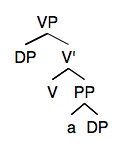
\includegraphics[width=\textwidth]{figures/sheehan-img001.png}

 
%%please move the includegraphics inside the {figure} environment
%%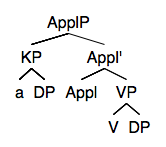
\includegraphics[width=\textwidth]{figures/sheehan-img002.png}

a.   b. 

On these (well-motivated) assumptions, there is al alternative reason that the PCC holds only in the presence of a dative clitic:  because this element serves to indicate the presence of an Applicative head. The presence of the clitic in (11c-d) therefore indicates a radically different underlying structure, which is not morphologically disambiguated in Italian, French and Catalan.\textstyleFootnoteSymbol{} \footnote{\citet{OrmazabalRomero2013} offer a different competition-based account of this pattern whereby the two a-marked DPs compete for the same Case position in spec vP. Space precludes a full discussion, but, while attractive, it seems that their account cannot be extended to the causative data to be discussed below, where the PCC holds with full DPs even in the absence of clitic doubling.} In order to ascertain whether the PCC is sensitive only to this structural difference or to the presence of the dative clitic itself, we need a context in which an indirect object marked with ‘a/à’ is not clitic doubled but cannot function as a locative. If the PCC holds in such contexts then we will know that the weak status of the indirect object is not crucial to the PCC. In the following section I show that the faire infinitive causative is such a context, and that in such cases the PCC can be observed to hold of all datives, not just clitics.

\section{The PCC in causatives} %3. /

A consideration of causatives shows that the PCC data for French, Italian and Catalan in ditransitive contexts are actually misleading. As \citet{Bonet1991} and others have noted, the PCC (somewhat unsurprisingly) also holds with dative clitic causees in the \textit{faire-infinitive} (\citealt{Postal1981}; \citealt{Quicoli1984}, \citealt{Rezac2008}):\footnote{I use the term ‘faire infinitive’ here to denote a particular kind of Romance causative, following \citet{Kayne1975}. Its crucial properties include: (i) dative on transitive causees, (ii) VS order for the caused event, (iii) causees which are agentive and (iv) causers which are not. Space precludes a discussion of minor differences between languages and I merely adopt the most uncontroversial account here, for expository reasons.} 

(\stepcounter{qwerty}{\theqwerty})  French (\citealt{Rezac2008}: 66, citing \citealt{Postal1981}, \citealt{Quicoli1984})

  *Je   vous     lui           laisserai   voir

    I      you.\textsc{acc}=     her.\textsc{dat=}   let.3\textsc{s}.\textsc{fut}    see

  Intended: ‘I will let her see you. 

As Bonet further notes, however, following \citet{Postal1989}, full DP datives are also banned in the presence of first/second person direct objects in this context in French:

(\stepcounter{qwerty}{\theqwerty})  French \citep[2]{Postal1989}

  a.  *Marcel vous   a   fait   épouser   au     médecin.

    Marcel   you.\textsc{acc}=  has   made   marry   to.the   doctor

    Intended: ‘Marcel had the doctor marry you.’

  b.   *On   nous     a   fait     choisir   à Jacques

    one     us.\textsc{acc} =has   made   choose   to Jacques

  Intended: ‘One/we had Jacques choose us.’

  c.   *On   vous   laissera   connaître   à Louise.

    one   you\textsc{.acc}=  let.\textsc{3s.fut} know     to Louise

    ‘We will let Louise meet you.

These kinds of examples contrast minimally with examples involving a 3\textsuperscript{rd} person direct object (even an animate one), which are fully grammatical, as Postal notes:

(\stepcounter{qwerty}{\theqwerty})  French \citep[2]{Postal1989}

  a.  Marcel   l’       a  fait    épouser   au     médecin.

    Marcel   her\textsc{.acc} =  has  made    marry   to.the   doctor

     ‘Marcel had the doctor marry her.’

b.   On   les       a   fait     choisir   à Jacques

    one   them.\textsc{acc}=  has   made   choose   to Jacques

   ‘We had Jacques choose them.’

Postal calls this the ‘Fancy Constraint’ and perhaps for this reason it is not usually discussed in connection with the PCC. It is, however, essentially a simpler version of the PCC, which we will call the ‘Simpler PCC’:

(\stepcounter{qwerty}{\theqwerty})  Simpler PCC (first version)

\begin{itemize}
\item \begin{itemize}
\item \begin{itemize}
\item \begin{itemize}
\item \begin{styleListParagraph}
In a combination of a direct object and dative in a causative construction, the direct object has to be third person.
\end{styleListParagraph}
\begin{styleListParagraph}
If the direct object is phonologically weak. 
\end{styleListParagraph}
\end{itemize}
\end{itemize}
\end{itemize}
\end{itemize}

I call \REF{ex:key:16} ‘simpler’ because it imposes no requirement on the status of the indirect object. This is the version of the PCC which holds also in Catalan and Italian causatives (the Catalan example is from Bonet and the Italian example from my own informants). 

(\stepcounter{qwerty}{\theqwerty})  Catalan \citep[195]{Bonet1991}

  *Em       van     fer     escollir   a   la   Teresa

    me.\textsc{acc}=  go.\textsc{3pl}   make   choose   to   the   Teresa

‘They made Teresa choose me.’

(\stepcounter{qwerty}{\theqwerty})  Italian 

  *Ti     ho     fatto   picchiare     a   mio   fratello

  You.\textsc{acc}  have.\textsc{1sg}   made beat         to   my   brother

    Intended: ‘I made my brother beat you.’

The same effect can be observed in Spanish (both Peninsular and Rioplatense), though it is more difficult to observe because of the additional availability of an ECM construction with these verbs (see \citealt{Strozer1976}, \citealt{Torrego2010}). Because of these complications, I discuss Spanish in a separate section below.  

As Postal also notes, the Fancy Constraint holds only where the causee is dative, and not where it is introduced by a preposition like \textit{par/de} or where no causee is overtly expressed:

(\stepcounter{qwerty}{\theqwerty})  French \citep[3]{Postal1989}

  a.   Marcel vous     a  fait   épouser   par   le   médecin.

    Marcel you.\textsc{acc}=  has  made   marry   by   the   doctor

    ‘Marcel had the doctor marry you.’

b.   On  nous     a   fait choisir.

    One   us.\textsc{acc}  =  has   made choose

    ‘One/we had us chosen.’

This is further potential evidence that we are dealing with the PCC. Though the structure of the \textit{faire-par} construction remains contested, there is widespread recognition that the ‘by phrase’ in examples like \REF{ex:key:19a} has adjunct-like properties and is not even projected in \REF{ex:key:19b} (see \citealt{Guasti1996}, \citealt{FolliHarley2007}, \citealt{SheehanCyrino2016} for recent discussion). In any case, evidence from binding shows that a by-phrase causee does not c-command the accusative object in the \textit{faire-par} construction, whereas a dative causee in the \textit{faire-infinitive} does, as \citet{Burzio1986} shows:

(\stepcounter{qwerty}{\theqwerty})  Italian \citep{Burzio1986} 

Ho   fatto   riparare   la   propria\textsubscript{i} macchina  a  Gianni\textsubscript{i}/*da   Gianni\textsubscript{i}

have.1S   made   repair   the  own   car   to   Gianni/  by   Gianni

‘I made Gianni repair his own car.’

In fact, there is evidence that in the \textit{faire-par} construction, c-command relations are reversed, with the accusative object binding into the by-phrase causee (\citealt{SheehanCyrino2016}):

(\stepcounter{qwerty}{\theqwerty})  Italian (\citealt{SheehanCyrino2016}: 286)

a.   Ho   fatto   leggere [  ogni   libro]\textsubscript{i} dal   suo\textsubscript{i}   autore. 

  have.1SG   made   read   each book   by.the   its   author  

  ‘I had each book read by its author.’

b.   *Ho   fatto   leggere   il  suo\textsubscript{i} libro   da   [ogni  autore]\textsubscript{i}

  have.1SG   made   read   the  his   book   by   each   author

It seems reasonable to assume, then, that the lack of PCC effects in such contexts can be attributed to the fact that the by phrase does not intervene (in c-command terms) between v and the accusative argument. 

The dative causee in the \textit{faire-infinitive,} however, is argument-like, obligatory and merged in a position which c-commands the accusative internal argument. This is reflected by the anaphor binding pattern in \REF{ex:key:20}. \citet{FolliHarley2007} propose that dative causees are merged in a righthand specifier of a lower vP, a proposal which I adopt here for ease of exposition, though other options are possible. In Italian and French, at least, all accusative and dative clitics must cliticise onto the causative verb (\citealt{Kayne1975}, \citealt{Burzio1986}, \citealt{Guasti1993}). If cliticization is mediated by Agree, as \citet{Preminger2019} claims, then a defective intervention configuration clearly arises as the FARE verb which I take to be an instance of a higher v, is clearly higher than the causee. The direct object clitic \textit{lo} is therefore c-commanded by v and ‘a Gianni,’ and ‘a Gianni’ is c-commanded by the higher FARE v, despite the unmarked word order:

(\stepcounter{qwerty}{\theqwerty})  Basic structure of faire-infinitive

 
%%please move the includegraphics inside the {figure} environment
%%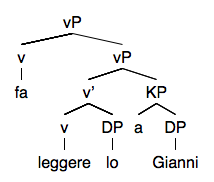
\includegraphics[width=\textwidth]{figures/sheehan-img003.png}

Postal proposes that, while the Fancy Constraint is widespread in French, it is not observed where the verbal complement of \textit{faire} is headed by \textit{connaître/reconnaître} or \textit{voir}, providing the following data:

(\stepcounter{qwerty}{\theqwerty})  French \citep[4]{Postal1989}

  a.   On   vous      fera         connaître   à Louise.

  one   you.\textsc{acc}=make.\textsc{3sg.fut}   know     to Louise

  ‘We made Louise meet you.’

b.   Jacques nous     a     fait   voir   à ses chefs

    Jacques us.\textsc{acc} =  has   made see   to his bosses

    ‘Jacques made his bosses see us.’

This is a potentially important distinction, which might shed important light on the nature of the PCC, if robust. Judgments on such are examples are varied, however and, although the effect might be less categorical than with other verbs, experimental results suggest that at least with \textit{voir}, the PCC still holds in its simpler form.

Given the sensitivity of judgments of this kind, 14 examples of this kind were included as fillers (with a parallel context) in a large online survey, taken by 42 people. Questions were presented in randomized order and rated on an 8-point scale from 0-7. Mean scores are given across participants. The results show a clear contrast: examples with 3rd person direct objects were clearly grammatical, receiving an average of acceptability of just under 5, regardless of the features of the indirect object \REF{ex:key:17}. Examples with two clitics received a slightly lower average mean \REF{ex:key:17b}, probably for processing reasons. All examples were presented along with a context (given in French) set in a busy classroom at the beginning of the school year:

(\stepcounter{qwerty}{\theqwerty})  French non-PCC contexts of \textit{faire-voir} ‘show’ 

  a.   La   professeure   \textbf{te/}  \textbf{lui/}  \textbf{me}     fait    

    the   teacher   you.\textsc{dat}/her.\textsc{dat}/me.\textsc{dat}= makes 

    voir \textbf{Jean},  qui   se   sent   nerveux. 

    see   Jean,   who \textsc{se}   feels   nervous

  ‘The teacher shows you/her/me Jean, who is feeling nervous.’        \textbf{[mean} \textbf{rating:} \textbf{4.98/4.86/4.62]}

b.   La   professeure   \textbf{me}   \textbf{le}  fait  voir.   

    the   teacher  me.\textsc{dat=}him.\textsc{acc=}  makes  see

    ‘The teacher shows me him.’   \textbf{[mean} \textbf{rating:} \textbf{4.45]}

This is as expected as these are non-PCC contexts in French because the direct object in all cases is 3\textsuperscript{rd} person. 

There is a clear contrast when we consider examples with 1st/2nd person direct object and a 3\textsuperscript{rd} person causee, the ‘strong PCC’ context. These were most unacceptable with dative clitics \REF{ex:key:25a}, but were also rated very low with full DP datives (an average of around 2 on the scale 8-point scale)(25b):

(\stepcounter{qwerty}{\theqwerty})  French PCC contexts of \textit{faire-voir} ‘show’

  a.   *Le professeur  \textbf{me/}   \textbf{te}       \textbf{lui}   fait   voir. 

    the   teacher  me.\textsc{acc/}  you.\textsc{acc}=  him.\textsc{dat}=  make see

Intended: ‘The teacher shows me/you to him.’

\textbf{[mean~ratings:} \textbf{0.49/0.50]}

  b.   *?La   professeure   \textbf{me/}    \textbf{te}       fait     voir 

    the     teacher     me.\textsc{acc}/  you.\textsc{acc=} makes   see 

à   Marie,  qui   se  sent   à   l’  aise. 

to Marie, who \textsc{se}   feels   at   the ease

Intended: ‘The teacher shows you to Marie, 

who is feeling at ease.’  \textbf{[mean~ratings:} \textbf{1.79/2.05]}

While further empirical investigation of the kinds of contrasts noted by Postal with individual verbs is clearly warranted, these initial experimental data suggest that the simpler PCC also holds with full dative DPs even where the embedded verb is \textit{voir}. 

The implication of the Catalan, Italian and French causative patterns is that the PCC in Romance languages is \textit{not} limited to contexts where the indirect object is a clitic or an element triggering morphological agreement. The languages in question fail to have clitic doubling of datives and yet the PCC still holds even where the dative is a full DP. In this way, the data show that the PCC holds wherever (i) the direct object has the relevant (language-specific) person/animacy feature; (ii) v establishes a detectable Agree relation with this direct object and (iii) an indirect object of any kind intervenes in that Agree relation. This can lead either to ungrammaticality (strong PCC) or interaction between phi-features (weak PCC).  

There is evidence that Postal’s Fancy Constraint is just the PCC from the kinds of repairs which are available in this context. Recall that in ditransitive contexts, changing a dative clitic into a tonic pronoun marked with a/à served to repair the PCC. In causative contexts, PCC violations can only be repaired by making the \textit{direct} object into a tonic pronoun:

(\stepcounter{qwerty}{\theqwerty})  French

Je   n’  ai   fait   frapper   que   toi   à   Jean

  I   \textsc{neg}   have   made   hit   but   you   to   Jean

  ‘I only made Jean hit YOU.’

(\stepcounter{qwerty}{\theqwerty})  Italian

Ho       fatto   picchiare   TE  a  mio  fratello

  have.\textsc{1sg}   made   beat      YOU  to  my  brother

  ‘I made my brother beat YOU.’

But, unlike in ditransitive contexts, changing the status of the dative does not help here: tonic pronouns are also banned in the presence of 1st/2nd person direct object clitics, just as full dative DPs are:

(\stepcounter{qwerty}{\theqwerty})  Italian\footnote{Another possible repair for some Italian speakers is to make the causee accusative, giving rise to an ECM-type complement without clitic climbing (\citealt{SchifanoSheehan2017}):

\begin{itemize}
\item \begin{styleListParagraph}
\%Lo/ *gli      fece      picchiarmi
\end{styleListParagraph}
\end{itemize}
    3sg.acc/  3sg.dat made    beat.inf.=1sg.acc      ‘She made him beat me’ECM is not usually possible with Italian FARE (but see \citealt{Burzio1986}, \citealt{SchifanoSheehan2017} for discussion). This repair is not possible with full DP causees, for unclear reasons, making it only partially parallel to what is described for Spanish below.} 

*Ti ho        fatto   picchiare   a    lui/LUI

  you have   made   beat     to him/HIM

  Intended: ‘I made him/HIM beat you.’

In sum, we have seen that a ‘simper PCC’ applies to causatives such that a 1\textsuperscript{st}/2\textsuperscript{nd} person direct object clitic is ruled out in the presence of any kind of dative in French, Italian and Catalan. Why do the data pattern differently in causative vs. ditransitive contexts? In ditransitive contexts we saw that, with the exception of Spanish (which has clitic doubling), no PCC effect was observed with full DP datives. In section 5, I propose that this is because ditransitives are structurally ambiguous in French, Italian and Catalan, just as they are in Spanish. As we saw for Spanish ditransitives, then, the PCC holds only where a DP is dative and not where it is locative. Before presenting this proposal, however, I discuss the behaviour of Spanish in causative contexts, as these data present additional complications, but essentially serve to reinforce the point being made. 

\section{Spanish causatives} %4. /

According to \citet{Torrego2010}, clitic doubling of datives in the faire-infinitive is optional, at least for some Spanish speakers (see also \citealt{Pineda2013} regarding ditransitives). I take the VS order in \REF{ex:key:29} to indicate that this is an instance of the \textit{faire} \textit{infinitive} nonetheless:

(\stepcounter{qwerty}{\theqwerty})  Spanish \citep[448]{Torrego2010}

La   entrenadora  (le)   hizo   repetir  el   ejercicio   a     la   atleta.

the   trainer   (her.\textsc{dat}=)   made   repeat  the   exercise   to   the  athlete

‘The trainer made the athlete repeat the exercise.’

In a PCC context then, a 1\textsuperscript{st}/2\textsuperscript{nd} person clitic is unsurprisingly ruled out in the presence of a clitic doubled dative. Note that this a spurious ‘se’ context in Spanish:

(\stepcounter{qwerty}{\theqwerty})  Spanish

*Marcelo   se   te   hizo   saludar  al   invitado.  

Marcelo   him.\textsc{dat}=  you.\textsc{acc}=  made   greet  to.the   guest

  ‘Intended: Marcelo made the guest greet you.’

What is more interesting, from our perspective, is what happens where the dative clitic is absent. Examples such as (31a-b) should be potentially ambiguous with either the clitic of the full DP functioning as the causee. This is because, as in the other Romance languages, 1\textsuperscript{st} and 2\textsuperscript{nd} person clitics are not morphologically distinguished for accusative and dative case and because, due to DOM, all animate internal arguments in Spanish are introduced by ‘a’.  In both cases, however, the 1st/2nd person clitic can only be construed as a dative causee, however:

(\stepcounter{qwerty}{\theqwerty})  Spanish

a.   Marcelo   te     hizo     ver   al   médico.

  Marcelo   you.*\textsc{acc/.dat=}  made  see     to.the   doctor

  (i) ‘Marcelo made you see the doctor.’

  (ii) *‘Marcelo made the doctor see you.’

b.   Nos     dejará   ver   a   Luisa.

  Us.*\textsc{acc/} \textsc{dat=}   let.\textsc{fut}  see   to   Luisa

  (i) ‘He made us see Luisa.’

  (ii) *‘He made Luisa see us.’

This is essentially the same effect described for Italian, French and Spanish: it is not possible to have a 1\textsuperscript{st}/2\textsuperscript{nd} person direct object in the presence of a dative argument. The only difference is that the presence of DOM means that the example is not ungrammatical, as the alternative reading in (i) is available. There is much more to be said about Spanish causatives, however. 

In addition to the faire infinitive, many varieties of Spanish appear to permit ECM complements of \textit{hacer} ‘make’. For our purposes, the relevant properties of this type of complement is that: (i) transitive causees can be realised as accusative clitics; (ii) SV order is observed in the caused event; (iii) clitic climbing is not possible (\citealt{Strozer1976}, \citealt{Treviño1992}, 1993, \citealt{Torrego2010}, Tubino \citealt{Blanco2011}). Consider the following examples by way of illustration of these properties in Mexican Spanish:

(\stepcounter{qwerty}{\theqwerty})  Mexican Spanish (\citealt{Treviño1992}: 311, 169)

a.   Juan lo     hizo   leer   estos libros.     

Juan him\textsc{.acc}=  made   read   these books

‘Juan made him read these books.’  

b.   Él  hizo  [  a   Sadat  exportarlas      desde   Francia].

He  made    to   Sadat  export.\textsc{inf}=them.\textsc{acc}   from   France

c.   *Él  las  hizo [  a   Sadat   exportar   desde   Francia].

  he them.\textsc{acc}=   made   to Sadat   export.\textsc{inf} from   France 

Once we accept that in Spanish, unlike in French, Italian and (for the most part) Catalan, an ECM-type of complement is available under the FARE cognate verb, some apparently quirky properties of Spanish causatives can be attributed to the PCC.\footnote{Actually a minority of Catalan speakers do seem to permit ECM under \textit{fer,} but this is certainly not a majority pattern (see Pineda, \citealt{SchifanoSheehan2018}).}  

First, consider the curious fact that animate direct object clitics cannot climb onto the causative verb in Spanish causatives (\citealt{Rivas1977}, \citealt{Bordelois1978}, \citealt{Torrego2010}):

(\stepcounter{qwerty}{\theqwerty})  Spanish \citep[463]{Torrego2010}

a.   *El   me     lo     hizo   saludar.

he   me.\textsc{dat} =  him.\textsc{acc} =  made greet

‘He made me greet him.’

b.   El   me     hizo   saludarlo.

he   me.\textsc{dat=}  made   greet=him.\textsc{acc}

In the current context, and bearing in mind the fact that Spanish displays PCC effects with animate direct objects, \REF{ex:key:33a} looks like a PCC effect. If this is the case, then it is not the clitic cluster that is a problem, nor the dative 1\textsuperscript{st} person clitic, but rather the animate direct object which attempts to Agree with \textit{hacer} ‘make’ past the dative causee.\footnote{As noted above a similar effect is attested with the 3\textsuperscript{rd} person masculine singular animate clitic \textit{le} in \textit{leísta} dialects of Spanish. I am not sure to what extent animate direct object clitics in non- \textit{leísta} dialects also trigger PCC effects with ditransitives.  } Example \REF{ex:key:33b} is grammatical, however, because it involves a more biclausal ECM construction in which the accusative clitic does not form an Agree dependency with \textit{hacer}, but rather with the lexical verb \textit{saludar}. As the causee asymmetrically c-commands this lexical verb, it does not function as an intervener in \REF{ex:key:33b}. 

  As this ECM causative is ‘biclausal’ in the relevant sense, it also fails to be subject to more standard PCC effects. Speakers of Latin American varieties of Spanish and many Peninsular varieties readily accept examples such as the following:

(\stepcounter{qwerty}{\theqwerty})  Spanish

a. (?)   Marcelo   hizo   al   invitado  saludarte.\\
    Marcelo   made  to.the   guest   greet=you.\textsc{acc}

    \textsc{‘}Marcelo made the guest greet you.’

b. (?) Dejará   a   Luisa   vernos.\\
      let.\textsc{fut}   to   Luisa   see=us.\textsc{acc}

  ‘They will let Luisa see us.’

These examples clearly have an interpretation whereby the 1\textsuperscript{st}/2\textsuperscript{nd} person clitic is construed as a direct object, as indicated in the gloss, and so there is no PCC effect in evidence. Again, this is because the direct object clitic does not agree with the matrix little v. In this way, PCC effects in Spanish causatives are more nuanced than in the other Romance languages under discussion. 

Now consider examples involving an animate direct object with DOM. As discussed above, these kinds of direct objects trigger PCC effects in Spanish ditransitives in the presence of clitic doubling, as discussed above. With causatives, the pattern is slightly different:

(\stepcounter{qwerty}{\theqwerty})  Spanish

  a.   *Ana   hizo   saludar   a   su   marido   al    invitado

    Ana   made   greet   to   her   husband  to.the   guest  

  b.   *Ana   le   hizo   saludar   a   su   marido   al   invitado

  Ana   him.dat   made   greet   to   her husband to.the   guest

c.   Ana   hizo     al     invitado   saludar   a   su   marido.

  Ana   made   to.the   guest   greet   to   her   husband

d.   \%Ana le   hizo   al   invitado saludar   a     su   marido.

  Ana   him.dat   made   to.the   guest   greet   to   her   husband

  ‘Ana made the guest greet her husband.’

If we take the basic position of the causee to indicate the difference between the faire-infinitive and ECM causatives, then these data show that PCC holds with DOM-marked full DP direct objects in the faire infinitive regardless of whether the indirect object is clitic doubled. In (35a-b), the VS order in the caused event indicates that this is an instance of the faire-infinitive, with clause union. For this reason, a DOM-marked direct object is not possible, by hypothesis, because the dative blocks agreement with the causative verb. Crucially, this is true not only in \REF{ex:key:35b}, where we see clitic doubling of the dative parallel to what we saw with ditransitives, but also in \REF{ex:key:31a}, where there is no dative clitic. This follows if, as noted above, clitic doubling is optional in the Spanish faire-infinitive (see also \citealt{Pineda2013}, who claims this is true also in Spanish ditransitives). Regardless of clitic doubling, then, the presence of a dative causee will trigger a PCC effect. As described in \REF{ex:key:12} above, in ditransitive constructions, a non-doubled indirect object has the option of being interpreted as a locative, and it is this fact which makes the presence of a clitic crucial to the PCC in this context. The same is not true in the faire infinitive, where DPs introduced by a/à always have the status of datives, base generated between the direct object and the causative v. 

Now consider (35c-d), which have SV order in the caused event and so can be taken to be instances of ECM causatives. All speakers accept \REF{ex:key:35c}, and this is as expected if this is a biclausal ECM context. Additionally, however, speakers from Argentina and certain parts of Spain also allow \REF{ex:key:35d}. In fact, these speakers also allow, even prefer, clitic doubling of the ECM causee with clitic direct objects, even in ‘strong PCC’ contexts, with 1\textsuperscript{st}/2\textsuperscript{nd} person direct objects:

(\stepcounter{qwerty}{\theqwerty})  Spanish 

a.   \%Marcelo   le   hizo   al   invitado saludarte.    Marcelo   him.\textsc{dat=}   made   to.the   guest  greet=you.\textsc{acc}

  ‘Marcelo made the guest greet you.’

b.   \%Clara   le   hizo   al   invitado   saludarlo.    \\
  Clara   him.\textsc{dat=} made   to.the   guest   greet=him.\textsc{acc}

    ‘Clara made the guest greet him.’

I leave open the status of the matrix dative clitic is in such examples. The fact that such examples are not subject to the PCC suggests that they cannot be instances of the faire-infinitive with a fronted causee. \citet{OrmazabalRomero2013} analyse them as instances of raising to object. It still remains unclear to me, however, how a dative clitic doubles an accusative causee (see also \citealt{OrdóñezSaab2018} for one proposal). What is clear from these data, however, despite the open questions, is that Spanish also displays PCC effects with both clitic and full DP datives, in parallel with the other Romance languages under discussion, once we control for the availability of ECM (or raising to object) complements.

\section{Theoretical implications} %5. /

Early approaches to the PCC characterised it as a morphological constraint (see \citealt{Bonet1991}, for example). More recently, however, significant challenges have been raised for this position (see \citealt{Preminger2019} for an overview), and the facts discussed here can be seen as further evidence that the PCC is not about morphology. In fact, the main aim of this chapter has been to show that the relevance of the PCC is \textit{not} limited to clitic clusters in Romance. As we have seen, when we consider Spanish DOM-marked direct objects and \textit{faire-infinitive} causatives, the PCC can be shown not to care about the weak/strong status of the indirect object. All that matters is the syntactic structure and the agreeing status of the direct object. 

While there have been many syntactic analyses of the PCC, most recent approaches reduce to the idea that it arises where “two arguments are in the domain of a single probing head” \citep[290]{Nevins2007}. A line of research stemming from Anagnostopoulou (2003, 2005) formalizes this in terms of defective intervention, whereby a probe attempts to agree with a goal with person features over a dative intervener (see \citealt{Anagnostopoulou2003}, 2005, \citealt{Nevins2007}, \citealt{Rezac2008}, \citealt{Preminger2019}). A distinct, but related approach, by \citet{AdgerHarbour2007} attributes the PCC to the fact that a single head with one set of person features cannot both agree with an animate [+participant] Theme and introduce an animate [+participant] argument in its specifier as these functions both require a distinct person feature. Note that, in their system, 3\textsuperscript{rd} person Themes are always [-participant], whereas animate recipients/benefactives are [+participant] even if they are 3\textsuperscript{rd} person.  Both kinds of approaches rely crucially on the fact that the direct object must Agree with a functional head. In the defective intervention approach, this is a head higher than the dative, such as v. In Adger and Harbour’s alterative account, it is Appl, the same head which introduces the applied argument. 

\citet{Bianchi2006} and \citet{Stegovec2017}, on the other hand, provide analyses which aim to capture the fact that (in ditransitives) the PCC only holds if both internal arguments are weak elements. In \citegen{Stegovec2017} approach, for example, weak arguments enter the derivation without a person feature and must receive one via agreement with a phase head. As the indirect object generally intervenes between the direct object and the phase head v, this leads to an intervention problem wherever both are weak 1\textsuperscript{st}/2\textsuperscript{nd} person pronouns. The Spanish data in ditransitives are already problematic for these latter kinds of accounts, as are the Romanian facts presented by Cornilescu (this volume, section 6), and the causative patterns show quite clearly that, in Romance at least, this kind of approach makes the wrong predictions. 

Mainstream accounts can, however, easily accommodate the Simpler PCC defended here. In the defective intervention approach, based on Anagnostopoulou (2003, 2005), \citet{BéjarRezac2003} and \citet{Rezac2008}, the PCC arises because a dative argument intervenes between a probe (v) and its [+person] goal, the accusative direct object:

(\stepcounter{qwerty}{\theqwerty})  v\textsubscript{[phi: ]}    > DP\textsubscript{DAT} >     DP\textsubscript{[+person]}

On this kind of approach, it is actually mysterious why the PCC would only apply to dative clitics. For the defective intervention account to extend to causatives, it has to be the case that the internal argument of the embedded predicate agrees with \textit{fare}, with the causee acting as an intervener:

(\stepcounter{qwerty}{\theqwerty})  fare\textsubscript{[phi: ]}   >  DP\textsubscript{DAT} >   DP\textsubscript{[+person]}

Given that internal arguments obligatorily cliticise onto \textit{faire}/\textit{fare} in both French and Italian, this kind of analysis seems promising. 

On Adger and \citegen{Harbour2007} approach, as noted above, the basic prediction is also that there would be no sensitivity to the clitic/non-clitic distinction, just as there is no sensitivity to the case-marking of the higher argument. For them, the PCC arises where a single head must both agree with the internal [+participant] direct object and introduce an animate [+participant] specifier:

(\stepcounter{qwerty}{\theqwerty})  *[\textsubscript{ApplP} DP\textsubscript{[+participant]} Appl … DP\textsubscript{[+participant]}]

\begin{styleNormalWeb}
This leads to ungrammaticality because a given head can only enter into an Agree relation with the same feature once, and the spec-head relation is conceived of as Agree-based. Whichever head introduces the causee in the faire infinitive: \textit{Appl} (\citealt{Ippolito2000}, \citealt{Ordóñez2008}, \citealt{Torrego2010}, \citealt{PitteroffCampanini2014}) or \textit{v} (\citealt{FolliHarley2007}), this head will be prevented from agreeing with a [+participant] Theme.\footnote{Note that it is more controversial to claim that the lowest direct object is Case-licensed by \textit{fare/faire}. \citet{BellettiRizzi2012} argue that it is, against Folli and \citegen{Harley2007} position that it is licensed low. The controversy relates partly to the status of passivisation of the faire-infinitive in Italian and French. As \citet{Preminger2019} shows, it is, in any case, possible, and probably necessary, to restate this kind of account without the need for abstract Case as long as cliticisation involves Agree.}   
\end{styleNormalWeb}

\begin{styleNormalWeb}
So why, then, does it appear to be the case that the PCC holds only where the dative is a clitic in ditransitive contexts in Romance? The answer, I propose, comes from the two potential structures for ditransitives and the fundamental ambiguity of \textit{a/à} as a dative/locative marker, discussed above in relation to Spanish. Following Holmberg, Sheehan and van der \citet{Wal2017} and \citet{Fournier2010}, we propose that (like Spanish) Catalan, Italian and French have two distinct structures for ditransitives (see \citealt{Demonte1995}, \citealt{Cuervo2003}, \citealt{Harley2002}, \citealt{HarleyMiyagawa2017}). These are as illustrated above by \REF{ex:key:12}, repeated here as \REF{ex:key:40}:
\end{styleNormalWeb}

(\stepcounter{qwerty}{\theqwerty})  Structures for the double object construction (a) and the prepositional dative (b)

 
%%please move the includegraphics inside the {figure} environment
%%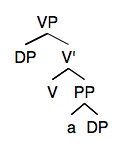
\includegraphics[width=\textwidth]{figures/sheehan-img001.png}

 
%%please move the includegraphics inside the {figure} environment
%%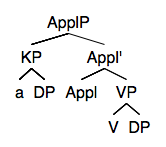
\includegraphics[width=\textwidth]{figures/sheehan-img002.png}

a.   b. 

In the extensive literature on the topic, it has been argued that many unrelated languages permit both kinds of structures, regardless of surface case morphology (see \citealt{Marantz1993}, \citealt{Pesetsky1995}, \citealt{Cuervo2003}, \citealt{Anagnostopoulou2003}, \citealt{Pylkkänen2002}, 2008, \citealt{MiyagawaTsujioka2004}, \citealt{Bruening2010}, \citealt{HarleyMiyagawa2017}). The issue remains contentious, however, as several of the other papers in this volume shows, see, especially, Calindro (this volume) and Cépeda \& Cyrino (this volume) on Brazilian Portuguese, Cornilescu (this volume) on Romanian, and Antonyuk (this volume) on Russian. If the Romance languages under discussion have two structures for distransitives, as outlined above, then PCC effects are predicted to hold only in structures like \REF{ex:key:40a} and not in those like \REF{ex:key:40b} (see \citealt{Rezac2008} on parallel contrasts in Basque). It is only in configurations like \REF{ex:key:40a} that the indirect object will function as an intervener. Where \textit{a/à} is the head of a locative PP which is base generated below the accusative direct object, no intervention effect will arise. 

In other words, it is this structural ambiguity in ditransitives which gives rise the false impression that the PCC only holds with dative clitics. Full DPs introduced by \textit{a/à} which occur with ditransitive verbs can be either dative or locative, having either the structure in \REF{ex:key:40a} or that in \REF{ex:key:40b}, whereas dative clitics are unambiguously dative, and so must derive from the structure in \REF{ex:key:40a}\footnote{For concreteness, I assume that clitics originate in argument positions, but there are other possibilities.} . Consider, by way of illustration, the French examples in \REF{ex:key:2}-(3) above, repeated here as (41a-b): 

(\stepcounter{qwerty}{\theqwerty})  French (\citealt{Kayne1975}: 173, 174)

  a.    *Paul   me       lui       présentera.

      Paul   me.\textsc{acc}=   him.\textsc{dat=} present.\textsc{3sg.fut}

    Intended: ‘Paul will introduce me to him.’

b.   Paul   me     présentera     à lui.

    Paul  me.\textsc{acc}=  present.\textsc{3s.fut}   to him

    ‘Paul will introduce me to him.’

Example \REF{ex:key:41a} is ungrammatical because it must have the structure in \REF{ex:key:40a}, whereby the dative intervenes between v and the direct object (in its base position). Example \REF{ex:key:41b}, however, is grammatical because it can be construed with the structure in \REF{ex:key:40b}. I assume that, with the structure in \REF{ex:key:40a}, it is also ungrammatical, in parallel with \REF{ex:key:41a}, and so only \REF{ex:key:40b} is possible (see also \citealt{Anagnostopoulou2003}, \citealt{Rezac2008} for similar proposals). 

Further support for this view comes from the fact that in French and Catalan the indirect object can be (exceptionally) realised as a locative clitic as a PCC repair strategy (see \citealt{Postal1990}, \citealt{Rezac2008}, on French; \citealt{Bonet1991}, 2007 on Catalan):

(\stepcounter{qwerty}{\theqwerty})  French

  \%  Paul   m’       y       présentera.

    Paul   me.\textsc{acc}=   there\textsc{=}   present.\textsc{3sg.fut}

  ‘Paul will introduce me to him.’

What is usual about such examples is that the locative clitics cannot unusually index animate arguments. Presumably, this is exceptionally permitted in such contexts to avoid ungrammaticality.

More generally, this proposal sheds new light on one of the main kinds of PCC repairs: they simply involve the prepositional dative construction not a PF repair. This explains immediately why there is no quantifier stranding in these instances (\citealt{Kayne1975}, \citealt{Rezac2008}):

(\stepcounter{qwerty}{\theqwerty})  French \citep[98]{Rezac2008}

  a.   Elle   la   leur   a   \textbf{tous}   présentée.

    she   her.\textsc{acc}=  them.\textsc{dat}   has   all   introduced 

  ‘She has introduced her to all of them.’ 

b.   Elle m'   a   (*tous)   présentée     à   eux. 

  she me.\textsc{acc}= has   all     introduced  to   them 

    ‘She has introduced me to (*all of) them.’~

Example \REF{ex:key:43a} shows that cliticization permits quantifier float. The fact that this is not possible in \REF{ex:key:43b} follows if this repair involves a different base generated structure, rather than a PF repair. 

In causative contexts, \textit{a/à} always indicates dative so these repairs are not possible, as noted above. This is because causees cannot be introduced as locatives headed by \textit{a/à}, presumably for semantic reasons. Note that they can be introduced as adjunct PPs, however (in the \textit{faire-par} construction) and this too is not subject to the PCC for parallel reasons: because the PP adjunct fails to intervene between the probe and the direct object. 

\section{Conclusions} %6. /

In this short article, I have argued that the PCC is simpler than previously thought. It blocks a 1st/2nd person direct object in the presence of any kind of intervening dative argument. The reason we observe PCC only with clitics in ditransitives is that \textit{a/à} is fundamentally ambiguous between being a locative and a dative marker and so only clitics are unambiguously dative.\footnote{A reviewer asks why the PCC does not hold optionally with full DPs even in ditransitive contexts. My claim is that it does but that this is not detectable as the locative repair is, in such cases, homophonous with the PCC-violating structure. In Spanish, where they are not homophonous, differences arise, as shown in \REF{ex:key:11} above.} \textsuperscript{} We have seen, furthermore, his is actually what is predicted by many, though not all, existing analyses of the PCC: any kind of dative will act as a defective intervener. In order for this to be the case, we must accept that there are two distinct structures for Romance ditransitives. While this has long been proposed for Spanish (\citealt{Demonte1995}, \citealt{Cuervo2003}), it remains more controversial for Italian, French and Catalan. Nonetheless, recent research has proposed, on a completely independent basis, that there are also two underlying structures for ditransitives in these languages. 

\textbf{Acknowledgements}

This research was partly funded by the British Academy. A version of this work was presented at Going \citealt{Romance2017} at University of Bucharest. Many thanks to everyone who offered feedback and critique. The usual disclaimers apply. 

\begin{verbatim}%%move bib entries to  localbibliography.bib

Adger, David \& Daniel Harbour. 2007. Syntax and Syncretisms of the Person Case Constraint. \textit{Syntax} 10(1): 2-37.

Albizu, Pablo. 1997. \textit{The} \textit{Syntax} \textit{of} \textit{Person} \textit{Agreement}. PhD thesis: USC.

Anagnostopoulou, Elena. 2003. \textit{The} \textit{Syntax} \textit{of} \textit{Ditransitives}. Berlin: Mouton de Gruyter.

Anagnostopoulou, Elena. 2005. Strong and weak person restrictions: a feature checking analysis. In Lorie Heggie \& Francisco Ordóñez (eds.), \textit{Clitic} \textit{and} \textit{affix} \textit{combinations:} \textit{theoretical} \textit{perspectives}, 199–235. Amsterdam: John Benjamins.

Béjar, Susana and Milan Rezac. 2003. Person licensing and the derivation of PCC effects. In Ana-Teresa Pérez-Leroux \& Yves Roberge (eds.), \textit{Romance} \textit{linguistics:} \textit{Theory} \textit{and} \textit{acquisition}, 49-62). Amsterdam: John Benjamins.

Belletti, Adriana and Luigi Rizzi. 2012. Moving verbal chunks in the low functional field. In Laura Brugè, Anna Cardinaletti, Giuliana Giusti, Nicola Munaro \& Cecilia Poletto (eds), \textit{Cartography} \textit{of} \textit{syntactic} \textit{structures} 7, 129-137. New York: Oxford University Press.

Bianchi, Valentina. 2006. On the syntax of person arguments. \textit{Lingua} 116: 2023-2067.

Bonet, Eulàlia. 1991. \textit{Morphology} \textit{after} \textit{syntax:} \textit{Pronominal} \textit{clitics} \textit{in} \textit{Romance.} Ph.D. thesis, MIT.

Bonet, E., 2007. The Person Case Constraint and repair strategies. In Roberta D’Alessandro, Susann Fischer, S. and Gunnar Hrafn Hrafnbjargarson (eds), \textit{Person} \textit{Restrictions,} 103-128. Berlin/New York: Mouton de Gruyter.

Bordelois, Ivonne. 1988. Causatives: From lexicon to syntax. \textit{Natural} \textit{Language} \textit{and} \textit{Linguistic} \textit{Theory} 6: 57-93.

Bruening, Benjamin. 2010. Double Object Constructions Disguised as Prepositional Datives. \textit{Linguistic} \textit{Inquiry} 41: 287-305.

Burzio, Luigi. 1986. \textit{Italian} \textit{syntax.} \textit{A} \textit{Government-Binding} \textit{approach}. Dordrecht: Reidel.

Cuervo, María Cristina. 2003. \textit{Datives} \textit{at} \textit{Large}, Ph.D. thesis, MIT. 

\citealt{Demonte1995}. Dative alternation in Spanish. \textit{Probus} 7: 5-30. 

Folli, Rafaela and Heidi Harley. 2007. Causation, Obligation, and Argument Structure: On the Nature of Little v. \textit{Linguistic} \textit{Inquiry} 38: 197-238.

Fournier, David. 2010. \textit{La} \textit{structure} \textit{du} \textit{prédicat} \textit{verbal} \textit{:} \textit{une} \textit{étude} \textit{de} \textit{la} \textit{construction} \textit{à} \textit{double} \textit{objet} \textit{en} \textit{français}. PhD thesis: University of Toronto.

Guasti, Maria Teresa. 1993. \textit{Causative} \textit{and} \textit{perception} \textit{verbs:} \textit{a} \textit{comparative} \textit{study}. Torino: Rosenberg \& Sellier.

Guasti, Maria Teresa. 1996. Semantic Restrictions in Romance Causatives and the Incorporation Approach. \textit{Linguistic} \textit{Inquiry} 27: 294-313.

Harley, Heidi. 2002. Possession and the Double Object Construction. \textit{Linguistic} \textit{Variation} \textit{Yearbook} 2: 29-68.

Harley, Heidi and Shigeru Miyagawa. 2017. Ditransitives. In \textit{Oxford} \textit{Research} \textit{Encyclopedia} \textit{of} \textit{Linguistics.} OUP.  DOI: 10.1093/acrefore/9780199384655.013.186

Haspelmath, Martin. 2004.  Explaining the ditransitive Person Case constraint: A usage-based approach. \textit{Constructions} 2. 

Holmberg, Anders, Michelle Sheehan \& Jenneke van der Wal. 2018.  Movement from the double object construction is not fully symmetrical To appear in \textit{Linguistic} \textit{Inquiry}. https://ling.auf.net/lingbuzz/003075 

Ippolito, Michela. 2000. Remarks on the argument structure of Romance causatives. Ms., MIT, Cambridge, MA.

 Kayne, Richard. 1975. \textit{French} \textit{syntax:} \textit{the} \textit{transformational} \textit{cycle}. Cambridge, MA: MIT Press.

Laka, Itziar. 1996. A brief grammar of Euskara, the Basque language. Open-access grammar, ISBN: 84-8373-850-3, Vitoria-Gasteiz: Euskal Herriko Unibertsitatea (University of the Basque Country). url: <http://www.ehu.eus/en/web/eins/basque-grammar>.

Marantz, Alec. 1993. Implications of asymmetries in double object constructions. In Sam A. Mchombo (ed.), \textit{Theoretical} \textit{aspects} \textit{of} \textit{Bantu} \textit{grammar}, 113-150. Stanford, CA: CSLI publications. 

Miyagawa, Shigeru \& Takae Tsujioka. 2004, Argument structure and ditransitive verbs in Japanese. \textit{Journal} \textit{of} \textit{East} \textit{Asian} \textit{Linguistics} 13(1): 1-38.

Nevins, Andrew Ira. 2007. The representation of third person and its consequences for Person-Case effects. \textit{Natural} \textit{Language} \textit{and} \textit{Linguistic} \textit{Theory} 25: 273–313.

Oehrle, Richard T. 1976. \textit{The} \textit{grammatical} \textit{status} \textit{of} \textit{the} \textit{English} \textit{dative} \textit{alternation}. PhD dissertation: MIT.

\begin{styleDefault}
Ordóñez, Francisco. 2008. Causativas y la distribución del sujeto causado en español: evidencia para un núcleo aplicativo. In \textit{X} \textit{Encuentro} \textit{Internacional} \textit{de} \textit{Lingüística} \textit{del} \textit{Noroeste}. Hermosillo, Sonora, México.
\end{styleDefault}

\begin{styleDefault}
Ormazabal, Javier and Juan Romero. 2007. The object agreement constraint. \textit{Natural} \textit{Language} \textit{and} \textit{Linguistic} \textit{Theory} 25: 315-347. 
\end{styleDefault}

\begin{styleDefault}
Ormazabal, Javier and Juan Romero. 2010. The derivation of dative alternations. In Maia Duguine, Susana Huidobro \& Nerea Madariaga (eds.), Ar\textit{gument} \textit{Structure} \textit{and} \textit{Syntactic} \textit{Relations} \textit{from} \textit{a} \textit{Crosslinguistic} \textit{Perspective}. 203-232. Amsterdam: John Benjamins. 
\end{styleDefault}

\begin{styleDefault}
Ormazabal, Javier and Juan Romero. 2013. Differential Object Marking, Case and Agreement. \textit{Borealis.} \textit{An} \textit{International} \textit{Journal} \textit{of} \textit{Hispanic} \textit{Linguistics} 2: 221-239.
\end{styleDefault}

Ordóñez, Francisco \& Andrés Saab. 2017. On the distribution of causee subjects in two Spanish dialects. \textit{Estudos} \textit{Linguísticos} \textit{e} \textit{Literários} 58: 186-209. 

Perlmutter, David. 1971. \textit{Deep} \textit{and} \textit{surface} \textit{structure} \textit{constraints} \textit{in} \textit{syntax}. New York: Reinhart and Winston Inc. 

Pesetsky, David. 1995. \textit{Zero} \textit{syntax:} \textit{Experiencers} \textit{and} \textit{cascades}. Cambridge, MA: MIT Press.

Pineda, Anna. 2013. Double object constructions in Spanish (and Catalan) revisited. In Sergio Baauw, Frank Drijkoningen, Luisa Meroni, Manuela Pinto (eds.), \textit{Romance} \textit{Languages} \textit{and} \textit{Linguistic} \textit{\citealt{Theory2011}: Selected papers from Going \citealt{Romance2011}}, 193-216. Amsterdam: John Benjamins. 

Pineda, Anna, Norma Schifano \& Michelle Sheehan. 2018. Transitivity in Catalan and Italian: evidence from causatives. Paper presented at \textit{Olinco}, Olomouc, Czech Republic. 

Pitteroff, Marcel \& Campanini, Cinzia. 2014. Variation in analytic causative constructions: a view on German and Romance. \textit{The} \textit{Journal} \textit{of} \textit{Comparative} \textit{Germanic} \textit{Linguistics} 16 (2-3): 209-230.

Postal, Paul M. 1981. A failed analysis of the French cohesive infinitive construction. \textit{Linguistic} \textit{Analysis} 8: 281-323.

Postal, Paul. M. 1989. \textit{Masked} \textit{inversion} \textit{in} \textit{French}. University of Chicago Press: Chicago. 

Postal, Paul. 1990. 1990. French indirect object demotion. In Paul Postal and Brian Joseph (eds.), \textit{Studies} \textit{in} \textit{Relational} \textit{Grammar} \textit{3}, 104-200. University of Chicago Press: Chicago.

Preminger, Omer. 2019. What the PCC tells us about “abstract” agreement, head movement, and locality. \textit{Glossa}, 4(1): 13. 

Pylkkänen, L. 2002. \textit{Introducing} \textit{Arguments}, MIT Ph.D Dissertation. 

Pylkkänen, Liina. 2008. \textit{Introducing} \textit{Arguments}. Cambridge, MA; London: MIT Press.

Quicoli, A. 1984. Remarks on French clitic systems. \textit{Linguistic} \textit{Analysis} 14: 55-95.

Rezac, Milan. 2008. The syntax of eccentric agreement: the Person Case Constraint and absolutive displacement in Basque. \textit{Natural} \textit{Language} \textit{and} \textit{Linguistic} \textit{Theory} 26: 61-106,

Rivas, Alberto M. 1977. \textit{A} \textit{Theory} \textit{of} \textit{Clitics}, MIT Ph.D Dissertation.  

Schifano, Norma and Michelle Sheehan. 2017. Italian faire-infinitives: the special case of \textit{volere}. To appear in Mirko Grimaldi, Rosangela Lai, Ludovico Franco and Benedetta Baldi (eds), \textit{Structuring} \textit{variation} \textit{in} \textit{Romance} \textit{linguistics} \textit{and} \textit{beyond}. Amsterdam: John Benjamins.

Sheehan, Michelle \& Sonia Cyrino. 2016. Variation and change in the faire-par causative. In Ernestina Carrilho, Alexandra Fieis, Maria Lobo \& Sandra Pereira (eds.), \textit{Romance} \textit{Languages} \textit{and} \textit{Linguistic} \textit{Theory}, 279-304. Amsterdam: John Benjamins.

Simpson, Jane \& Meg Withgott. 1986. Pronominal Clitic Clusters and Templates. In Hagit Borer (ed.), \textit{The} \textit{syntax} \textit{of} \textit{pronominal} \textit{clitics}, 149-174. Orlando: Academic Press.

Stegovec, Adrian. 2017. Between you and me: Two cross-linguistic generalizations on person restrictions. In Aaron Kaplan, Abby Kaplan, Miranda K. McCarvel, \& Edward J. Rubin (eds.), \textit{Proceedings} \textit{of} \textit{the} \textit{34th} \textit{West} \textit{Coast} \textit{Conference} \textit{on} \textit{Formal} \textit{Linguistics}, 498-508. Somerville, MA: Cascadilla Proceedings Project.

Strozer, Judith R. 1976. \textit{Clitics} \textit{in} \textit{Spanish}, PhD dissertation: UCLA.

Torrego, Esther. 2010. Variability in the case patterns of causative formation in romance and its implications. \textit{Linguistic} \textit{Inquiry} 41: 445-470.

Treviño, Esthela. 1992. Subjects in Spanish causative constructions. In \textit{Romance} \textit{Languages} \textit{and} \textit{Modern} \textit{Linguistic} \textit{Theory}, eds.  Hirschbüler, P. \& Koerner, E., 309-324.

Treviño, Esthela. 1993. \textit{Las} \textit{causativas} \textit{del} \textit{español} \textit{con} \textit{complemento} \textit{infinitivo}. El Colegio de México, DF.

Tubino Blanco, Mercedes. 2011. \textit{Causatives} \textit{in} \textit{Minimalism}. Amsterdam: John Benjamins.


\end{verbatim}
\sloppy\printbibliography[heading=subbibliography,notkeyword=this]\end{document}
